\section{Introduction}

[TO DO]

\paragraph{Characteristics of J1331: Lensing}
\begin{itemize}
\item at redshift $z_d\simeq0.113$ [TO DO: REF]
\item large reddish bulge
\item superimposed by quadruplet of extended bluish images at a redshift of $z_s\simeq0.254$ [TO DO: REF]
\item lensed object might be a star-forming blob of a background galaxy.
\end{itemize}

\paragraph{Data used}
\begin{itemize}
\item Hubble Space Telescope (HST) imaging by \cite{SWELLSI}
\end{itemize}


[TO DO]


%============================================================================


\begin{figure*}
\centering
\begin{subfigure}{.5\textwidth}
  \centering
  \includegraphics[width=.9\linewidth]{fig/first_glimpse_450.ps}
  \caption{J1331 in F450W ("blue")}
  \label{fig:???}
\end{subfigure}%
\begin{subfigure}{.5\textwidth}
  \centering
  \includegraphics[width=.9\linewidth]{fig/first_glimpse_814.ps}
  \caption{J1331 in F814W ("red")}
  \label{fig:???}
\end{subfigure}
\begin{subfigure}{.5\textwidth}
  \centering
  \includegraphics[width=.9\linewidth]{fig/lens_imgpos.ps}
  \caption{The lensing images}
  \label{fig:lens_just_imgpos}
\end{subfigure}%
\begin{subfigure}{.5\textwidth}
  \centering
  \includegraphics[width=.9\linewidth]{fig/stellar_kinematics_data.ps}
  \caption{Stellar Kinematics by \citet{SWELLSV}}
  \label{fig:???}
\end{subfigure}
\caption{Hubble Space telescope (HST) images and stellar kinematics of the galaxy SDSS J1331+3638 (J1331), which has a large counter-rotating core and whose bulge acts as a strong lens for a bluish background source. \emph{Panel (a) and (b):} HST images of J1331 by \citet{SWELLSI} in two filters, F450W in panel (a) and F814W in panel (b). The galaxy's coordinates on the sky are right ascension $\alpha$ = 202.91800$^\circ$ and declination $\delta$ = 36.46999$^\circ$ (epoch J2000). Image orientation and scaling are indicated in panel (a); the scaling transformation from arcseconds to the physical size of the galaxy in kpc uses the galaxy's redshift $z_d = 0.113$ \citep{SWELLSIII}. The black solid line in panel (a) shows the orientation of the major-axis. The line has a length of 10 arcsec and indicates the region within which we carry out the Jeans modelling. (NOT ALL THE TIME.???????) \emph{Panel (c):} The central region of J1331 in F450W, surface brightness subtracted. An IRAF ellipse ???? fit to the F450W surface brightness in panel (a) was subtracted from the image. The (smoothed) residuals within the white square in panel (a) are shown in panel (c). Four bright blobs (A,B,C and D) become visible, which are arranged in a typical strong lensing configuration around the center of the galaxy (G). \emph{Panel (d):} Stellar Kinematics along the galaxy's major axis as measured by \citet{SWELLSV}, line-of-sight rotation velocity $v_\text{rot}$, line-of-sight velocity dispersion $\sigma$ and the rms-velocity $v_\text{rms} = \sqrt{v_\text{rot}^2 + \sigma^2}$. The dotted line in panel (b) indicates the galaxy's effective half-light radius (in the F814W filter), $R_\text{eff} = 2.6" = 5.2$ kpc. The $v_\text{rot}$ curve reveals that J1331 is counter-rotating within $R_\text{eff}$. TO DO: Add (x,y) axis in figure b).???????}
\label{fig:specialJ1331}
\end{figure*}

\clearpage
